\documentclass[11pt]{amsart}
\usepackage[margin=1.15in]{geometry}
\usepackage{amssymb,mathtools}
\usepackage{booktabs}
\usepackage{tikz}
\usepackage{listings}
\usepackage[hidelinks]{hyperref}
\usepackage{xurl}

\lstset{basicstyle=\ttfamily\scriptsize,columns=fullflexible,keepspaces=true,
  breaklines=true,frame=none,xleftmargin=1em,upquote=true}

\newtheorem{theorem}{Theorem}
\newtheorem{proposition}[theorem]{Proposition}
\newtheorem{lemma}[theorem]{Lemma}
\newtheorem{corollary}[theorem]{Corollary}
\theoremstyle{definition}
\newtheorem{definition}[theorem]{Definition}
\theoremstyle{remark}
\newtheorem{remark}[theorem]{Remark}

\newcommand{\R}{\mathbb{R}}
\newcommand{\Z}{\mathbb{Z}}
\newcommand{\Q}{\mathbb{Q}}
\newcommand{\C}{\mathbb{C}}
\newcommand{\diam}{\operatorname{diam}}
\newcommand{\conv}{\operatorname{conv}}
\newcommand{\repo}{\url{https://github.com/alonamit1729/affinemess-applets}}

\title{The largest planar seven-distance sets}

\author{Alon Amit}
\author{Claude (Anthropic)}

\date{18 November 2026}

\begin{document}

\begin{abstract}
Let $g(k)$ be the largest number of points in the plane that determine at most $k$ distinct distances. We
prove that $g(7)=16$, and that up to similarity there are exactly two sixteen-point sets with at most seven
distances. Both are pieces of the triangular lattice, which confirms for $k=7$ the conjecture of Erdős and
Fishburn that maximum $k$-distance sets with $k\ge7$ are pieces of the triangular lattice. The proof is
computer-assisted and self-contained. The main steps of the proof
are a complete list of the $228$ distance patterns of ten-point planar sets with at most six distances (a
number first obtained by Szöllősi and Östergård), in which every pattern discarded along the way
carries a polynomial identity that certifies its impossibility; an exact determination of all
realisations of these patterns; a diameter-graph argument showing that every sixteen-point set with at
most seven distances contains such a ten-point set, including a new elementary proof that thirteen
points whose diameter graph is a $13$-cycle and which determine at most seven distances form a regular
$13$-gon; and an exhaustive extension search in exact arithmetic. The same methods show that there are
exactly sixteen fifteen-point sets with at most seven distances, one of which is not contained in a
sixteen-point set.
\end{abstract}

\maketitle

\section{Introduction}

For a finite set $X\subset\R^2$ let $\Delta(X)=\{|x-y| : x,y\in X,\ x\neq y\}$ be the set of distances it
determines, and let
\[
  g(k)=\max\{|X| : X\subset\R^2,\ |\Delta(X)|\le k\}.
\]
Erdős and Fishburn \cite{EF} introduced this function and determined it for $k\le5$:
$g(1)=3$, $g(2)=5$, $g(3)=7$, $g(4)=9$ and $g(5)=12$. Wei \cite{W} proved $g(6)=13$, and Szöllősi and
Östergård \cite{SO} classified the maximum six-distance sets. Erdős and Fishburn exhibited
sixteen-point sets with seven distances, and conjectured that for $k\ge7$ every maximum $k$-distance set
is similar to a subset of the triangular lattice \cite{EF}. Partial results towards $g(7)=16$ were
obtained by Budianto \cite{B}, and Bao and Yu \cite{BY} determined, for $7\le k\le34$, the largest
$k$-distance subsets of the triangular lattice that use the $k$ smallest lattice distances.

We write points of the plane as complex numbers, put $\omega=e^{i\pi/3}$, and use triangular coordinates:
$(a,b)\in\Z^2$ stands for the lattice point $a+b\omega$, whose squared length is $a^2+ab+b^2$. Let
\[
  H=\{(a,b)\in\Z^2 : a^2+ab+b^2\in\{0,1,3\}\},
\]
the thirteen lattice points at squared distance $0$, $1$ or $3$ from the origin, and
\[
  E_1=H\cup\{(-2,0),(-2,2),(0,-2)\},\qquad E_2=H\cup\{(-2,0),(0,2),(2,-2)\}.
\]
Both sets have sixteen points and the same seven squared distances $1,3,4,7,9,12,13$. They are not
similar: the squared distance $4$ occurs $20$ times in $E_1$ and $18$ times in $E_2$
(Figure~\ref{fig:E}).

\begin{theorem}\label{thm:main}
\leavevmode
\begin{enumerate}
\item Every set of points in the plane that determines at most seven distinct distances has at most
  sixteen points. Hence $g(7)=16$.
\item Every set of sixteen points in the plane that determines at most seven distinct distances is
  similar to $E_1$ or to $E_2$.
\end{enumerate}
\end{theorem}

In particular $g(7)=16$, and since $E_1$ and $E_2$ are pieces of the triangular lattice, the conjecture of
Erdős and Fishburn stated above holds for $k=7$.

The same methods also classify the fifteen-point sets with seven distances: there are sixteen of them up to
similarity, and one is not contained in a sixteen-point set (Theorem~\ref{thm:15} in
Section~\ref{sec:fifteen}).

\begin{figure}[t]
\centering
\begin{tikzpicture}[scale=0.62]
\def\pts#1{\foreach \a/\b in {#1} {\fill (\a+0.5*\b, 0.8660254*\b) circle (3.2pt);}}
\def\extra#1{\foreach \a/\b in {#1} {\filldraw[fill=white,line width=1pt] (\a+0.5*\b, 0.8660254*\b) circle (3.8pt);}}
\begin{scope}
  \foreach \a in {-3,...,3} \foreach \b in {-3,...,3} {
    \pgfmathsetmacro{\x}{\a+0.5*\b}\pgfmathsetmacro{\y}{0.8660254*\b}
    \pgfmathparse{abs(\x)<3.3 && abs(\y)<2.7 ? 1 : 0}
    \ifnum\pgfmathresult=1 \fill[gray!45] (\x,\y) circle (1pt);\fi}
  \pts{0/0,1/0,0/1,-1/1,-1/0,0/-1,1/-1,1/1,-1/2,-2/1,-1/-1,1/-2,2/-1}
  \extra{-2/0,-2/2,0/-2}
  \node at (0,-2.6) {$E_1$};
\end{scope}
\begin{scope}[xshift=8cm]
  \foreach \a in {-3,...,3} \foreach \b in {-3,...,3} {
    \pgfmathsetmacro{\x}{\a+0.5*\b}\pgfmathsetmacro{\y}{0.8660254*\b}
    \pgfmathparse{abs(\x)<3.3 && abs(\y)<2.7 ? 1 : 0}
    \ifnum\pgfmathresult=1 \fill[gray!45] (\x,\y) circle (1pt);\fi}
  \pts{0/0,1/0,0/1,-1/1,-1/0,0/-1,1/-1,1/1,-1/2,-2/1,-1/-1,1/-2,2/-1}
  \extra{-2/0,0/2,2/-2}
  \node at (0,-2.6) {$E_2$};
\end{scope}
\end{tikzpicture}
\caption{The two sixteen-point sets with seven distances. The thirteen black points form $H$; the three
hollow points differ. Grey dots are other points of the triangular lattice.}
\label{fig:E}
\end{figure}

The upper bound $g(7)\le16$ follows from the method of part (2) without knowing the two sets
(Proposition~\ref{prop:extend}); Corollary~\ref{cor:17} gives a second, direct argument.

\subsection*{Outline}
The proof follows the strategy of Erdős and Fishburn and of Wei: remove points until the largest distance
disappears, and study the remaining set, which has fewer distances. Section~\ref{sec:reduction} shows
that every sixteen-point set with at most seven distances contains ten points with at most six
distances, a \emph{core}. Sections~\ref{sec:patterns}--\ref{sec:realisations} determine all ten-point sets
with at most six distances: they have one of $228$ distance patterns (a number first stated by Szöllősi and
Östergård \cite{SO}), each pattern has finitely many
realisations, and up to similarity there are $257$ such sets. Section~\ref{sec:extensions} finds every way
of adding six points to a core without exceeding seven distances, and Section~\ref{sec:end} identifies the
results.

Three ingredients deserve mention.
\begin{itemize}
\item The list of $228$ patterns is derived by generating patterns one point at a time. A pattern is
  discarded only together with a \emph{certificate}: a polynomial identity which shows, by multiplying
  out, that no planar point set has this pattern (Section~\ref{sec:patterns}). There are $527{,}338$
  certificates. The number $228$ agrees with Table~9 of \cite{SO}, which was obtained by Gröbner-basis
  computations; we do not use that table.
\item The reduction to ten points needs one geometric lemma about thirteen points whose diameter graph is
  a cycle. We give an elementary proof (Lemma~\ref{lem:C13}).
\item All computations are exact: integers, rational numbers and algebraic numbers represented in
  number fields, with signs of real algebraic numbers certified by isolating intervals with rational
  endpoints. No floating-point number takes part in a decision.
\end{itemize}

\subsection*{Software and data}
Everything needed to check the proof is in the folder \texttt{tools/16-7-proof} of the repository
\repo{}; the version described here is commit \texttt{e10d2f9}. It contains a Jupyter notebook
\texttt{two-shapes.ipynb} that carries out or checks every step in about three and a half minutes using
only Python and SymPy, the programs \texttt{certificates/generate.py} and \texttt{certificates/check.py}
discussed in Section~\ref{sec:patterns}, and the lists of patterns. The two large certificate files
($0.22$ GB compressed) are attached to the release \texttt{certificates-v1} of the same repository. A
rendered version of the notebook is at \url{https://affinemess.com/16-7-proof.html}.
Section~\ref{sec:computation} lists exactly what the proof takes from the literature and from computation.

\section{Distance patterns and certificates}\label{sec:defs}

\subsection{Patterns}
Let $p_0,\dots,p_{n-1}$ be distinct points in the plane. Colour each pair $\{i,j\}$ so that two pairs get
the same colour exactly when $|p_i-p_j|$ is the same. The resulting colouring of the edges of the complete
graph $K_n$, up to renaming the colours, is the \emph{distance pattern} of the points. Two colourings are
\emph{equivalent} if one becomes the other after renumbering the vertices and renaming the colours. A
pattern is \emph{realisable} if it is the pattern of some planar point set. Every sub-pattern (the
colouring induced on a subset of the vertices) of a realisable pattern is realisable.

Equivalence is decided by a canonical form, computed by individualisation and refinement in the manner of
nauty \cite{MP}: the canonical form of a colouring is the lexicographically smallest colour sequence over
the vertex orderings produced by a search tree whose branching does not depend on the given numbering.

\subsection{Squared lengths and the Gram matrix}
Let a pattern on $n$ points have colours $0,\dots,k-1$, and write $c(i,j)$ for the colour of the pair
$\{i,j\}$. Introduce one variable $x_c$ for each colour, to stand for the squared distance of that colour.
For a base point $b$ and $i,j\neq b$ put
\[
  G^b_{ij}=x_{c(b,i)}+x_{c(b,j)}-x_{c(i,j)}\quad(i\neq j),\qquad G^b_{ii}=2x_{c(b,i)}.
\]
If points $p_0,\dots,p_{n-1}$ realise the pattern and $x_c$ is the squared distance of colour $c$, then
$G^b_{ij}=2\langle p_i-p_b,\,p_j-p_b\rangle$. So $G^b$ is twice the Gram matrix of $n-1$ vectors in $\R^2$,
it has rank at most $2$, and every $3\times3$ minor of $G^b$ vanishes. The minors are cubic polynomials in
the $x_c$ with integer coefficients.

\subsection{Certificates}

\begin{definition}\label{def:cert}
A \emph{certificate} for a pattern with colours $0,\dots,k-1$ is an identity in the
polynomial ring $\Z[x_0,\dots,x_{k-1}]$ of the form
\begin{equation}\label{eq:cert}
  d\cdot\prod_{c}x_c^{e_c}\prod_{a\neq b}(x_a-x_b)^{e_{ab}} \;=\; \sum_{i}A_i\,M_i,
\end{equation}
where $d$ is a non-zero integer, the exponents $e_c,e_{ab}$ are non-negative integers, each $M_i$ is a
$3\times3$ minor of one of the matrices $G^b$, and each $A_i$ is a polynomial with integer coefficients.
\end{definition}

\begin{lemma}\label{lem:cert}
A pattern that has a certificate is not realisable.
\end{lemma}

\begin{proof}
Suppose points realise the pattern, and substitute their squared distances for the $x_c$. Every minor
$M_i$ vanishes, so the right side of \eqref{eq:cert} is $0$. On the left, $d\neq0$, every $x_c$ is
positive because the points are distinct, and $x_a\neq x_b$ for $a\neq b$ because different colours stand
for different distances. So the left side is not $0$.
\end{proof}

Checking a certificate means expanding both sides of \eqref{eq:cert} and comparing coefficients; the
minors are recomputed from the pattern. Two examples, writing $M_b(r;s)$ for the minor of $G^b$ with rows
$r$ and columns $s$: four points at mutual distance $x_0$ have the certificate $4x_0^3=M_0(123;123)$; and
for the five-point pattern in which the four pairs through point $0$ have colour $0$ and the other six
pairs colour $1$, one certificate is
\[
  18\,x_0^3 = 13\,M_0(123;123)-3\,M_1(234;234)-22\,M_0(123;124).
\]
Here the multipliers are constants. Certificates with a product of degree $d$ on the left have multipliers
of degree $d-3$.

\section{Ten points with six distances: the 228 patterns}\label{sec:patterns}

\subsection{Generation one point at a time}
We construct lists $L_4,L_5,\dots,L_{10}$, where $L_n$ is a set of patterns on $n$ points with at most six
colours (up to equivalence). Call a pattern $Q$ on $n$ points with at most six colours a
\emph{candidate} at level $n$ if $n=4$, or if $n\ge5$ and every sub-pattern of $Q$ on $n-1$ points is
equivalent to a member of $L_{n-1}$. The list $L_n$ consists of the candidates at level $n$ that are kept:
a candidate is discarded only if it has a certificate.

This scheme is the one used by Szöllősi and Östergård \cite{SO}, who discarded a candidate when a Gröbner
basis showed that its equations have no solution with non-zero, pairwise different squared lengths, not
even a complex one. We replace this criterion by certificates, which are easier to check and do not
depend on the correctness of a Gröbner-basis implementation.

\begin{proposition}[computer-assisted]\label{prop:lists}
There are lists $L_4,\dots,L_{10}$ such that, for each $n$, every candidate at level $n$ either belongs to
$L_n$ or has a certificate. The numbers are given in Table~\ref{tab:levels}; in particular $|L_{10}|=228$.
\end{proposition}

\begin{table}[ht]
\centering
\begin{tabular}{@{}lrrrrrrr@{}}
\toprule
$n$ & 4 & 5 & 6 & 7 & 8 & 9 & 10\\
\midrule
candidates & 25 & 1{,}193 & 537{,}230 & 14{,}732 & 1{,}565 & 635 & 228\\
discarded, each with a certificate & 1 & 271 & 517{,}001 & 10{,}065 & 0 & 0 & 0\\
kept: $|L_n|$ & 24 & 922 & 20{,}229 & 4{,}667 & 1{,}565 & 635 & 228\\
\quad with at most five colours & 23 & 678 & 1{,}620 & 398 & 157 & 57 & 19\\
\quad with six colours & 1 & 244 & 18{,}609 & 4{,}269 & 1{,}408 & 578 & 209\\
\midrule
certificates with product of degree 3 & 1 & 237 & 380{,}254 & 10{,}065 & & & \\
\phantom{certificates with product of degree} 4 & & 34 & 135{,}749 & & & & \\
\phantom{certificates with product of degree} 5 & & & 998 & & & & \\
\bottomrule
\end{tabular}
\caption{The generation of patterns with at most six colours. At four points the only discarded pattern
is the one-coloured one. The rows of candidates and kept patterns agree with Table~9 of \cite{SO}.}
\label{tab:levels}
\end{table}

\begin{proposition}\label{prop:A}
Every set of ten points in the plane with at most six distances has one of the $228$ patterns of
$L_{10}$.
\end{proposition}

\begin{proof}
We show by induction on $n=4,\dots,10$ that every set $X$ of $n$ points with at most six distances has its
pattern in $L_n$. The pattern of $X$ is realisable, so it has no certificate (Lemma~\ref{lem:cert}). For
$n=4$ it is a candidate by definition, hence in $L_4$. For $n\ge5$, every subset of $n-1$ points of $X$
has at most six distances, so by induction its pattern is in $L_{n-1}$; thus the pattern of $X$ is a
candidate, and having no certificate, it is in $L_n$ by Proposition~\ref{prop:lists}.
\end{proof}

\subsection{How Proposition~\ref{prop:lists} is verified}\label{sec:verify-lists}
Proposition~\ref{prop:lists} contains two computational claims: that the candidates at each level are
listed completely, and that each discarded candidate has a valid certificate.

\emph{Certificates.} The program \texttt{check.py} reads a pattern and a certificate, recomputes the
relevant minors from the pattern, expands both sides of \eqref{eq:cert} as dictionaries of integer
coefficients and compares them. Its core is about fifty lines of Python using only integer arithmetic; it
is printed in Appendix~\ref{app:check}. All $527{,}338$ certificates pass it; the check takes about $45$
core-minutes. The $272$ certificates at four and five points are in the repository, and the notebook
checks them together with random samples of $400$ and $200$ certificates at six and seven points on every
run.

\emph{Candidates.} The program \texttt{generate.py} lists the candidates at level $n$ from $L_{n-1}$. For
each $Q\in L_{n-1}$ it adds a new point and colours the $n-1$ new pairs one at a time, using the colours of
$Q$ and new colours up to six in all, with new colours introduced in order. After each new pair it tests
every sub-pattern that has just become complete: for sub-patterns on at most six points by looking up a
table of all labelled colourings equivalent to members of $L_4$, $L_5$, $L_6$, and on more points by
canonical form. A partial colouring is abandoned as soon as such a test fails. Nothing is lost by this
pruning, because the lists are closed under taking sub-patterns: a sub-pattern on $s$ points of a candidate
at level $n$ is in $L_s$ (by induction on $n-s$). Every candidate $P$ at level $n$ is found, because
deleting any vertex $v$ of $P$ leaves a member $Q$ of $L_{n-1}$, and the colours of the pairs at $v$ form
one of the colourings tried for $Q$. The program then checks that each candidate is in $L_n$ or is the
pattern of a certificate. The whole run for $n=5,\dots,10$ takes about $13$ minutes on two cores, and
reproduces the first three rows of Table~\ref{tab:levels} exactly.

The candidates had first been listed by a different program, which shares no code with
\texttt{generate.py} and takes its canonical forms from nauty. At six points, where $98\%$ of the
certificates are, a third enumeration that tries every colouring of the five new pairs without any pruning
gives the same $537{,}230$ candidates.

\emph{How the certificates were found} plays no role in the proof. For each candidate, the degree-$d$
part of the ideal generated by the minors was computed by linear algebra modulo a large prime, all products
of $d$ factors $x_c$ and $x_a-x_b$ were tested for membership at once ($d=3,4,5$), and the multipliers were
then solved for exactly over $\Q$ and scaled to integers.

\section{Realisations of the 228 patterns}\label{sec:realisations}

Let $P\in L_{10}$ have $k$ colours, and fix the colour of the pair $\{0,1\}$ as the unit: its squared length
is $1$, and the other $k-1$ squared lengths are unknowns. A \emph{solution} of $P$ is an assignment of
non-zero, pairwise different complex values to these unknowns at which the $84$ principal minors of $G^0$
vanish (the minors with rows and columns $\{i,j,l\}$, $1\le i<j<l\le9$; each says that the points
$0,i,j,l$ are coplanar).

\begin{proposition}[computer-assisted]\label{prop:B}
Every pattern in $L_{10}$ has finitely many solutions, $282$ in all. Every solution is real, and is
realised: there are points $p_0,\dots,p_9$ in the plane with pattern $P$ whose squared distances are the
given values. Consequently every set of ten points in the plane with at most six distances is similar to
one of $282$ explicitly known point sets.
\end{proposition}

The solutions are computed as follows. Let $q$ be the product of all unknowns and of all differences
between two squared lengths. A Gröbner basis of the minors together with $wq-1$, where $w$ is an auxiliary
variable, describes exactly the solutions (a solution with $q=0$ does not extend to $w$, one with $q\neq0$
extends uniquely). In every case the basis has finitely many solutions; a lexicographic basis is obtained
by the FGLM algorithm and the solutions are listed by means of a primitive element, as tuples of elements
of number fields $\Q(t)=\Q[T]/(f)$ with $f$ irreducible. For each real root of $f$ the points are then
rebuilt in exact coordinates in $\Q(t)$, using the basis given by two of the position vectors; the
Euclidean condition (positive squared lengths and a positive definite Gram matrix of the basis) is
decided with certified signs, and all $45$ squared distances are compared with the solution.

The second half of Proposition~\ref{prop:B} (every solution is realised) is verified directly and
independently of how the solutions were found. The first half, that there are no further solutions,
depends on the correctness of the Gröbner-basis computation, done with SymPy \cite{sympy}. It was
cross-checked with a different implementation (FLINT), using the equations of all $210$ quadruples of
points; the solution sets agree for all $228$ patterns (folder \texttt{flint-check}).

Table~\ref{tab:solutions} summarises the result. For $199$ patterns the solution is unique and rational.
The other $29$ patterns have irrational squared lengths, in $\Q(\sqrt3)$ or $\Q(\sqrt5)$ for $21$ of them
and in fields of degree $3$ to $6$ for the remaining eight, which include the fields of the regular
$9$-, $11$- and $13$-gons. All $228$ patterns are rigid.

\begin{table}[ht]
\centering
\begin{tabular}{@{}lrrrrrr@{}}
\toprule
solutions per pattern & 1 & 2 & 3 & 4 & 5 & 6\\
number of patterns & 199 & 20 & 1 & 3 & 2 & 3\\
\midrule
degree of the number field & 1 & 2 & 3 & 4 & 5 & 6\\
number of Galois orbits of solutions & 199 & 22 & 1 & 2 & 2 & 3\\
\bottomrule
\end{tabular}
\caption{The $282$ solutions of the $228$ patterns. A Galois orbit of degree $e$ consists of $e$ solutions,
one for each root of $f$; all roots are real.}
\label{tab:solutions}
\end{table}

\begin{corollary}\label{cor:257}
Up to similarity there are exactly $257$ sets of ten points in the plane with at most six distances:
$19$ with five distances and $238$ with six.
\end{corollary}

Different solutions can give similar point sets, because a solution is tied to a numbering of the points.
Similarity is decided by comparing the sorted lists of ratios of squared lengths, identified as real
algebraic numbers by their minimal polynomials and isolating intervals, together with the canonical form
of the pattern in which every colour is named by the rank of its length.

\section{The reduction to ten points}\label{sec:reduction}

\subsection{Diameter graphs}
Let $X$ be a finite set in the plane with diameter $D$. The \emph{diameter graph} of $X$ joins two points at
distance $D$. Let $X_D$ be the set of points on at least one of its edges and $m=|X_D|$.

\begin{lemma}\label{lem:diam}
\leavevmode
\begin{enumerate}
\item Every point of $X_D$ is a vertex of $\conv X$; in particular $X_D$ is in strictly convex position.
\item Any two edges of the diameter graph meet, at a common endpoint or at a point interior to both.
\item The diameter graph has at most one cycle. If its restriction to $X_D$ is not a single cycle through
  all $m$ points, it has an independent set of size at least $\lceil m/2\rceil$ in $X_D$. If it is a single
  cycle, $m$ is odd.
\end{enumerate}
\end{lemma}

\begin{proof}
(1) If $|p-q|=D$, then $X$ lies in the closed disc of radius $D$ about $q$ and $p$ is on its boundary circle.
A point of a disc on the boundary circle is not a convex combination of other points of the disc.

(2) is due to Hopf and Pannwitz \cite{HP}. Let $pq$ and $rs$ be edges with four distinct endpoints. By (1)
the four points are in strictly convex position. If the segments did not cross, $pq$ and $rs$ would be
opposite sides of a convex quadrilateral, whose diagonals have total length greater than $|pq|+|rs|=2D$;
so some distance would exceed $D$.

(3) is Lemmas 3--5 and 9 of \cite{W}. A cycle of odd length $m$ has an independent set of size $(m-1)/2$.
\end{proof}

If $I\subseteq X_D$ is independent in the diameter graph, then $A=I\cup(X\setminus X_D)$ does not contain two
points at distance $D$. If $X$ has at most seven distances, $A$ has at most six, and $|A|=|X|-m+|I|$.

\subsection{Points on the hull}
We use a classical theorem on convex polygons.

\begin{theorem}[Altman \cite{A}; Fishburn \cite{F}; see also {\cite[Lemma 2]{EF}}]\label{thm:altman}
The vertices of a convex polygon with $h$ vertices determine at least $\lfloor h/2\rfloor$ distances. If they
determine exactly $\lfloor h/2\rfloor$, the polygon is regular when $h$ is odd, and is regular or a regular
$(h+1)$-gon with one vertex removed when $h\ge8$ is even.
\end{theorem}

\begin{lemma}\label{lem:hull}
Let $X$ be a finite set with at most seven distances whose convex hull has $h\ge14$ vertices. Then $X$
consists of these vertices, and it is a regular $15$-gon, a regular $14$-gon, or a regular $15$-gon with
one vertex removed. In particular, if $|X|\ge15$ and $X$ is not a regular $15$-gon, then $\conv X$ has at most
thirteen vertices and $m\le13$.
\end{lemma}

\begin{proof}
Let $h$ be the number of vertices of $\conv X$. By Theorem~\ref{thm:altman}, $\lfloor h/2\rfloor\le7$, so
$h\le15$. Suppose $h\ge14$. The vertices determine at least seven distances, hence exactly seven, the
distances of $X$. By Theorem~\ref{thm:altman} they form a regular $15$-gon, a regular $14$-gon, or a regular
$15$-gon with one vertex $v_0$ removed. Scale so that the circumradius is $1$ and the centre is $0$.
Suppose that $X$ has a point $q$ that is not a vertex; it lies in the polygon, so $r=|q|<1$.

The point $q$ is not the centre: its distance to the vertices would be $1$, and a chord $2\sin(\pi j/n)$ of a
regular $n$-gon equals $1$ only if $n=6j$, while $n\in\{14,15\}$. So every circle about $q$ meets the
circumcircle in at most two points, and each distance from $q$ to the vertices occurs at most twice. If
$h=15$, $q$ has at least eight distances to the vertices, too many. If $h=14$, the fourteen distances from $q$
take each of the seven distances of $X$ exactly twice, so
\[
  \sum_{v}|q-v|^2 = 2S,
\]
where $S$ is the sum of the seven squared distances, that is, of the squared chord lengths $4\sin^2(\pi j/n)$,
$1\le j\le7$, with $n=14$ or $15$. Using $4\sin^2\theta=2-2\cos2\theta$ one finds $S=16$ for $n=14$ and
$S=15$ for $n=15$. On the other hand $\sum_v|q-v|^2=14(1+r^2)-2\,q\cdot\sum_v v$. For the regular $14$-gon
$\sum_v v=0$, so $14(1+r^2)=32$ and $r^2=9/7>1$. For the regular $15$-gon minus $v_0$, $\sum_v v=-v_0$, so
$7r^2+q\cdot v_0=8$; but $7r^2+q\cdot v_0\le7r^2+r<8$. Both are impossible, so $X$ has no point
besides the vertices. For the last sentence, $|X|=h\le15$ would force $X$ to be a regular $15$-gon; so
$h\le13$, and $m\le h$ by Lemma~\ref{lem:diam}(1).
\end{proof}

\subsection{Thirteen points with a cyclic diameter graph}
\begin{lemma}\label{lem:C13}
Let $Y$ be a set of thirteen points in the plane that determines at most seven distances and whose
diameter graph is a cycle through all thirteen points. Then $Y$ is the vertex set of a regular $13$-gon.
\end{lemma}

\begin{proof}
Scale so that the diameter is $1$. By Lemma~\ref{lem:diam}(1), $Y$ is in strictly convex position; label
its points $p_0,\dots,p_{12}$ counterclockwise around the boundary of $\conv Y$, indices modulo $13$. We use
repeatedly that from each vertex $p_y$ the rays to $p_{y+1},p_{y+2},\dots,p_{y+12}$ appear in
counterclockwise order and span an angle less than $\pi$.

\emph{Step 1: the diameters.} Let $\{p_x,p_y\}$ be a diameter. Removing $p_x$ and $p_y$ from the cycle leaves
a path through the other eleven points. Each edge of the path is a diameter disjoint from $\{p_x,p_y\}$, so
by Lemma~\ref{lem:diam}(2) it crosses the segment $p_xp_y$ and has its endpoints on opposite sides of the
line $p_xp_y$. Hence the path alternates between the two sides, which therefore contain six and five of
its points. The two sides of this line contain the two boundary arcs strictly between $p_x$ and $p_y$, so
$y-x\equiv\pm6\pmod{13}$. Each point has two neighbours in the cycle, so $p_y$ is joined exactly to
$p_{y+6}$ and $p_{y+7}=p_{y-6}$.

\emph{Step 2: monotone chains.} For every $y$ and $1\le k\le5$,
\begin{equation}\label{eq:chain}
  |p_y-p_{y+k}|<|p_y-p_{y+k+1}|.
\end{equation}
Indeed, $p_{y+k+7}$ is at distance $1$ from both $p_{y+k}$ and $p_{y+k+1}$, so it lies on the perpendicular
bisector $\ell$ of the side $p_{y+k}p_{y+k+1}$. The line $\ell$ meets the polygon in the segment from the
midpoint of that side to $p_{y+k+7}$, whose interior lies in the interior of the polygon (the two endpoints
are not on a common side). So the vertices $p_{y+k+8},\dots,p_{y+k+13}=p_{y+k}$ lie strictly
on the same side of $\ell$ as $p_{y+k}$. Among them is $p_y$ (as $8\le13-k\le12$), and points on that side
are closer to $p_{y+k}$ than to $p_{y+k+1}$.

Call $\{p_y,p_{y+k}\}$ ($1\le k\le6$) a chord of \emph{step} $k$; every pair is a chord of exactly one step.
By \eqref{eq:chain}, for each $y$ the six numbers $|p_y-p_{y+k}|$, $k=1,\dots,6$, are distinct distances of
$Y$, in increasing order, the last being $1$. So $Y$ has six or seven distances. If it has exactly six, $\delta_1<\dots<\delta_6=1$,
then every chord of step $k$ has length $\delta_k$. If it has seven, $\delta_1<\dots<\delta_7=1$, then
$|p_y-p_{y+k}|$, the $k$-th smallest of six distinct elements of $\{\delta_1,\dots,\delta_7\}$, is
$\delta_k$ or $\delta_{k+1}$, so
\begin{equation}\label{eq:twovalues}
  \text{for each } k\le5, \text{ the chords of step } k \text{ take at most two values.}
\end{equation}

\emph{Step 3: apex angles.} For each $y$ let $\gamma_y$ be the angle at $p_y$ of the isosceles triangle
$p_yp_{y+6}p_{y+7}$, whose legs have length $1$. Its base is a side of the polygon, hence shorter than $1$,
so $0<\gamma_y<\pi/3$. Let $w_y=p_{y+6}-p_y$, a unit vector. By the ordering of rays,
$p_{y+7}-p_y=e^{i\gamma_y}w_y$. Since $p_{(y+7)+6}=p_y$, also $p_{y+7}-p_y=-w_{y+7}$, so
\begin{equation}\label{eq:w}
  w_{y+7}=-e^{i\gamma_y}\,w_y\qquad(y\in\Z/13).
\end{equation}
The side from $p_j$ to $p_{j+1}$ is the base of the triangle with apex $p_{j+7}$:
\[
  p_{j+1}-p_j=(p_{j+1}-p_{j+7})-(p_j-p_{j+7})=(e^{i\gamma_{j+7}}-1)\,w_{j+7}
  =2\sin\tfrac{\gamma_{j+7}}2\cdot ie^{i\gamma_{j+7}/2}\,w_{j+7}.
\]
So the side $p_jp_{j+1}$ has length $s(\gamma_{j+7})$, where $s(t)=2\sin(t/2)$, and direction
$\tau_j=ie^{i\gamma_{j+7}/2}w_{j+7}$. By \eqref{eq:w}, $w_{j+1}=w_{j+14}=-e^{i\gamma_{j+7}}w_{j+7}$ and
$w_{j+8}=-e^{i\gamma_{j+1}}w_{j+1}=e^{i(\gamma_{j+1}+\gamma_{j+7})}w_{j+7}$, hence
\[
  \tau_{j+1}/\tau_j=\exp\Bigl(i\bigl(\gamma_{j+1}+\tfrac12(\gamma_{j+7}+\gamma_{j+8})\bigr)\Bigr).
\]
The exterior angle of the polygon at $p_{j+1}$ lies in $(0,\pi)$ and is congruent modulo $2\pi$ to the
exponent, which also lies in $(0,\pi)$ because every $\gamma<\pi/3$. So the exterior angle at $p_j$ is
\begin{equation}\label{eq:ext}
  \varepsilon_j=\gamma_j+\tfrac12(\gamma_{j+6}+\gamma_{j+7}).
\end{equation}
Summing over $j$ gives $2\pi=2\sum_y\gamma_y$, so $\sum_y\gamma_y=\pi$.

\emph{Step 4: equal sides.} If all sides are equal, all $\gamma_y$ are equal (as $s$ is injective on
$(0,\pi/3)$), so by \eqref{eq:ext} all exterior angles are equal. A convex polygon with equal sides and equal
angles is regular, and we are done. This covers the case of six distances, so from now on $Y$ has seven
distances and not all sides are equal. The sides are chords of step $1$, so they take exactly two values, and
the $\gamma_y$ take two values $\alpha<\beta$. Let $n_\alpha$ and $n_\beta$ be the numbers of $\gamma_y$ equal to
$\alpha$ and to $\beta$; then $n_\alpha,n_\beta\ge1$, $n_\alpha+n_\beta=13$ and
$n_\alpha\alpha+n_\beta\beta=\pi$, so $\alpha<\pi/13<\beta$.

Arrange the angles in the cyclic sequence $\gamma_0,\gamma_7,\gamma_{14},\dots$, in which $\gamma_y$ is
followed by $\gamma_{y+7}$. Words such as $\alpha\beta\alpha$ below refer to consecutive terms of this cyclic
sequence.

\emph{Step 5: two chord formulas.} For the chord of step $5$ from $p_x$, note that
$p_{x+5}-p_x=w_x+w_{x+6}+w_{x+12}$. By \eqref{eq:w}, $w_{x+6}=-e^{-i\gamma_{x+6}}w_x$ and
$w_{x+12}=-e^{-i\gamma_{x+12}}w_{x+6}$, so with $A=\gamma_{x+6}$ and $B=\gamma_{x+12}$, two consecutive terms
of the sequence,
\[
  |p_x-p_{x+5}|^2=\bigl|1-e^{-iA}+e^{-i(A+B)}\bigr|^2
  =1-8\sin\tfrac A2\,\sin\tfrac B2\,\cos\tfrac{A+B}2=:f(A,B).
\]
For the chord of step $2$ from $p_{j-1}$, the vector $p_{j+1}-p_{j-1}$ is the sum of the
sides from $p_{j-1}$ to $p_j$ and from $p_j$ to $p_{j+1}$. They have lengths $s(\gamma_{j+6})$ and
$s(\gamma_{j+7})$, and the angle between them is $\varepsilon_j$. With $(A,B,C)=(\gamma_{j+6},\gamma_j,\gamma_{j+7})$, three consecutive terms of the
sequence,
\[
  |p_{j-1}-p_{j+1}|^2=s(A)^2+s(C)^2+2s(A)s(C)\cos\bigl(B+\tfrac{A+C}2\bigr)=:F(A,B,C).
\]
As $x$ and $j$ run over $\Z/13$, these formulas cover all pairs and all triples of consecutive terms.

\emph{Step 6: not both $\alpha\alpha$ and $\beta\beta$.} Suppose both words $\alpha\alpha$ and $\beta\beta$
occur. Then $n_\alpha,n_\beta\ge2$, so $2\alpha+\beta<n_\alpha\alpha+n_\beta\beta=\pi$, and also
$\alpha+2\beta<\pi$ (if $n_\beta=2$ then $\alpha+2\beta=\pi-(n_\alpha-1)\alpha$; if $n_\beta\ge3$ then
$2\beta<2\pi/3$ and $\alpha<\pi/13$). For fixed $a$,
$\sin\frac x2\cos\frac{a+x}2=\frac12\bigl(\sin(x+\frac a2)-\sin\frac a2\bigr)$, so
\[
  f(\alpha,\alpha)-f(\alpha,\beta)=4\sin\tfrac\alpha2\bigl(\sin(\beta+\tfrac\alpha2)-\sin\tfrac{3\alpha}2\bigr),\quad
  f(\alpha,\beta)-f(\beta,\beta)=4\sin\tfrac\beta2\bigl(\sin\tfrac{3\beta}2-\sin(\alpha+\tfrac\beta2)\bigr).
\]
Both are positive, since $\sin\phi>\sin\psi$ whenever $0<\psi<\phi$ and $\psi+\phi<\pi$; here
$\psi+\phi$ is $2\alpha+\beta$ and $\alpha+2\beta$ respectively. So the chords of step $5$ take the three different
values $f(\alpha,\alpha)>f(\alpha,\beta)>f(\beta,\beta)$, contradicting \eqref{eq:twovalues}. Since $13$ is
odd, the sequence cannot alternate, so exactly one of the words $\alpha\alpha$, $\beta\beta$ occurs.

\emph{Step 7: properties of $F$.} Clearly $F(A,B,C)$ is symmetric in $A$ and $C$, and
\begin{equation}\label{eq:Fa}
  F(A,B,A)=2s(A)^2\bigl(1+\cos(A+B)\bigr)=4s(A)^2\cos^2\tfrac{A+B}2.
\end{equation}
Moreover, at any point with $A+C<\pi$ and $\varepsilon:=B+\frac{A+C}2\le\frac\pi2$,
\[
  \frac{\partial F}{\partial C}=2\cos\tfrac C2\bigl(s(C)+s(A)\cos\varepsilon\bigr)-s(A)s(C)\sin\varepsilon
  \ \ge\ s(C)\Bigl(2\cos\tfrac C2-2\sin\tfrac A2\Bigr)\ >\ 0,
\]
because $\cos\varepsilon\ge0$, $\sin\varepsilon\le1$ and $\frac C2<\frac\pi2-\frac A2$. By symmetry the same
holds for $\partial F/\partial A$.

\emph{Step 8: no two $\beta$'s adjacent.} Then every $\beta$ is between two $\alpha$'s, so
$n_\beta\le6$ and $n_\alpha\ge7$. The word $\alpha\beta\alpha$ occurs. The $\alpha$'s form $n_\beta$ runs
of consecutive terms; as $n_\alpha>n_\beta$, some run has length at least $2$, and it is followed by a
$\beta$, so $\alpha\alpha\beta$ occurs. If all runs had length $2$ we would have $13=3n_\beta$; so some run
has length $1$ or at least $3$, and $\beta\alpha\beta$ or $\alpha\alpha\alpha$ occurs. Now
\[
  F(\alpha,\beta,\alpha)<F(\alpha,\alpha,\alpha)<F(\alpha,\alpha,\beta),\qquad\text{and if }
  n_\beta\ge2,\quad F(\alpha,\alpha,\beta)<F(\beta,\alpha,\beta).
\]
The first inequality is \eqref{eq:Fa}, as $\alpha<\frac{\alpha+\beta}2<\frac\pi2$. For the second, increase
$C$ from $\alpha$ to $\beta$ in $F(\alpha,\alpha,C)$: here $\alpha+C\le\alpha+\beta<\pi$ and
$\varepsilon\le\frac{3\alpha+\beta}2<\frac\pi2$, since $3\alpha+\beta<n_\alpha\alpha+n_\beta\beta=\pi$.
For the third (needed only when $\beta\alpha\beta$ occurs, so that $n_\beta\ge2$), increase $A$ from
$\alpha$ to $\beta$ in $F(A,\alpha,\beta)$: here $A+\beta\le2\beta<\pi$ and
$\varepsilon\le\alpha+\beta<\frac\pi2$, since $2\alpha+2\beta<n_\alpha\alpha+n_\beta\beta$. So the three
words found give three different values of chords of step $2$, contradicting \eqref{eq:twovalues}.

\emph{Step 9: no two $\alpha$'s adjacent.} Then $n_\alpha\le6$, $n_\beta\ge7$ and $\beta<\pi/7$. The word
$\beta\alpha\beta$ occurs; $\beta\beta\alpha$ occurs because some run of $\beta$'s has length at least $2$;
and $\alpha\beta\alpha$ or $\beta\beta\beta$ occurs because not all runs of $\beta$'s have length $2$. Now
\[
  F(\alpha,\beta,\alpha)<F(\beta,\beta,\alpha)<F(\beta,\beta,\beta)<F(\beta,\alpha,\beta).
\]
The first two inequalities follow from Step 7 (increase $A$, then $C$, from $\alpha$ to $\beta$ with
$B=\beta$; throughout $A+C\le2\beta<\pi$ and $\varepsilon\le2\beta<\frac\pi2$), the last from
\eqref{eq:Fa}, as $\frac{\alpha+\beta}2<\beta<\frac\pi2$. Again three different values of chords of step $2$
occur, a contradiction.

So the sides are all equal, and $Y$ is a regular $13$-gon by Step 4.
\end{proof}

\subsection{Cores}
\begin{proposition}\label{prop:core}
Every set $X$ of sixteen points in the plane with at most seven distances contains ten points with at most
six distances.
\end{proposition}

\begin{proof}
By Lemma~\ref{lem:hull}, $m\le13$. If the diameter graph restricted to $X_D$ is not a single cycle through
$X_D$, Lemma~\ref{lem:diam}(3) gives an independent set $I$ with $|I|\ge\lceil m/2\rceil$, and
$A=I\cup(X\setminus X_D)$ has $16-m+|I|\ge16-\lfloor m/2\rfloor\ge10$ points and at most six distances. If it
is a single cycle and $m\le11$, then $m$ is odd and taking every other point of the cycle gives
$|A|=16-m+\frac{m-1}2=16-\frac{m+1}2\ge10$. If it is a single cycle and $m=13$, then $X_D$ is a set of thirteen
points with at most seven distances whose diameter graph is a $13$-cycle, so by Lemma~\ref{lem:C13} it is a
regular $13$-gon. A regular $13$-gon has six distances, so any ten of its vertices will do.
\end{proof}

A ten-point subset of $X$ with at most six distances is called a \emph{core} of $X$. By
Propositions~\ref{prop:A} and~\ref{prop:B}, every core is similar to one of the $282$ point sets of
Section~\ref{sec:realisations}.

\section{Extending a core}\label{sec:extensions}

\begin{proposition}[computer-assisted]\label{prop:extend}
Let $K$ be one of the $282$ ten-point sets of Proposition~\ref{prop:B}. No set of seventeen points with at
most seven distances contains $K$. If a set $X$ of sixteen points with at most seven distances contains $K$,
then the seven squared distances of $X$ are proportional to $1,3,4,7,9,12,13$.
\end{proposition}

The proof is a finite search, which we now describe. Let $\Delta$ be the set of squared distances of $K$; by
Proposition~\ref{prop:B}, $|\Delta|\in\{5,6\}$. If $X\supset K$ has at most seven distances, at most
$b=7-|\Delta|\in\{1,2\}$ new squared distances (not in $\Delta$) occur in $X$ altogether; we call $b$ the
\emph{budget}.

\emph{Candidate points.} Let $y\in X\setminus K$. Among its ten squared distances to $K$, at most $b$ values
are new. If some value occurs three times, $y$ is the circumcentre of three points of $K$, necessarily not
collinear. Otherwise every value occurs at most twice, so at most $2b$ of the ten distances are new and at
least $10-2b\ge6$ points of $K$ are at squared distances in $\Delta$ from $y$. The computation shows that no
core has more than five collinear points. Fix a family $\mathcal T$ of non-collinear triples of points of
$K$ such that every set of $10-2b$ points of $K$ contains a triple of $\mathcal T$ (chosen greedily; all
$120$ triples would also do). If $y$ has squared distances $r,s,t\in\Delta$ to a triple $(u,v,w)$, then
subtracting $|y-u|^2=r$ from $|y-v|^2=s$ and from $|y-w|^2=t$ gives two independent linear equations,
\[
  2\langle y,v-u\rangle=|v|^2-|u|^2+r-s,\qquad 2\langle y,w-u\rangle=|w|^2-|u|^2+r-t,
\]
which determine $y$. So $y$ belongs to the finite set consisting of the circumcentres of non-collinear
triples of $K$ and the solutions of these equations for $(u,v,w)\in\mathcal T$ and $(r,s,t)\in\Delta^3$ that
also satisfy $|y-u|^2=r$. Each such point is kept as a candidate if its squared distances to $K$ contain at
most $b$ new values. For one core it was checked that using all $120$ triples gives the same candidates.

\emph{Compatible sets.} A depth-first search adds candidates one at a time, maintaining the set of new
squared distances (to $K$ and among the added points), and abandons a branch as soon as this set has more
than $b$ elements. It lists every set of candidates that can be added to $K$ within the budget.

\emph{Exactness.} The coordinates of $K$ lie in the number field of its solution, and all candidates have
coordinates in the same field. The search uses only field operations and tests of equality (of two squared
distances, or of a determinant with $0$). Such a computation has the same outcome at every embedding of the
field into $\R$, so it is run once for each of the $229$ Galois orbits of solutions.

\emph{Result.} The largest number of points that each of the $282$ cores reaches is as follows.
\begin{center}
\begin{tabular}{@{}lrrrrrrr@{}}
\toprule
largest number of points reached & 10 & 11 & 12 & 13 & 14 & 15 & 16\\
number of cores & 11 & 10 & 18 & 28 & 18 & 12 & 185\\
\bottomrule
\end{tabular}
\end{center} The cores that reach sixteen points have $185$ different patterns, and there
are $826$ ways in all to complete them (counted with the core fixed). In every one of them the seven squared
distances are proportional to $1,3,4,7,9,12,13$. No core reaches seventeen points. The search takes under a
minute.

\section{The sixteen-point sets}\label{sec:end}

\begin{proposition}[computer-assisted]\label{prop:palette}
Up to congruence, there are exactly two sets of sixteen points in the plane all of whose squared distances lie
in $\Pi=\{1,3,4,7,9,12,13\}$, namely $E_1$ and $E_2$.
\end{proposition}

\begin{proof}
Such a set $Z$ is not collinear, since sixteen collinear points have fifteen distances from an endpoint. So
it contains three non-collinear points; label them $z_0,z_1,z_2$ so that their squared distances
$a=|z_0-z_1|^2$, $b=|z_0-z_2|^2$, $c=|z_1-z_2|^2$ satisfy $a\le b\le c$, all in $\Pi$. Every other point of
$Z$ has squared distances $(r,s,t)\in\Pi^3$ to $z_0,z_1,z_2$ and, as in Section~\ref{sec:extensions}, is
determined by them. So for each triangle shape $(a,b,c)$ there are at most $7^3$ candidate points, and $Z$
consists of the triangle and $13$ candidates that are pairwise at squared distances in $\Pi$. A clique
search over the candidates, for all triangle shapes, finds exactly two sets up to congruence (congruence is
decided by the canonical form of the table of squared distances), and they are congruent to $E_1$ and $E_2$.
The computation is exact, in rational coordinates with respect to the basis $z_1-z_0$, $z_2-z_0$, and takes
a few seconds.
\end{proof}

\begin{proof}[Proof of Theorem~\ref{thm:main}]
(2) Let $X$ be a set of sixteen points with at most seven distances. By Proposition~\ref{prop:core} it has a
core, which by Propositions~\ref{prop:A} and~\ref{prop:B} is similar to one of the $282$ sets $K$. Applying the
similarity, $X$ contains $K$, so by Proposition~\ref{prop:extend} its squared distances are proportional to
those of $\Pi$. After scaling, Proposition~\ref{prop:palette} shows that $X$ is congruent to $E_1$ or $E_2$.

(1) Let $X$ have seventeen points and at most seven distances. A sixteen-point subset $X'$ has a core $K'$,
similar to one of the sets $K$ of Proposition~\ref{prop:B}; then a set similar to $X$ contains $K$, which
contradicts Proposition~\ref{prop:extend}. Hence $g(7)\le16$, and $E_1$ shows $g(7)=16$.
\end{proof}

The bound $g(7)\le16$ also follows directly from part (2):

\begin{corollary}\label{cor:17}
Neither $E_1$ nor $E_2$ can be extended by a point without creating an eighth distance.
\end{corollary}

\begin{proof}
Let $y$ be a point at squared distances $r,s,t\in\Pi$ from the lattice points $0$, $1$ and $\omega$, which
belong to both sets. Writing $y=a+b\omega$ with $a,b$ real, the linear equations of
Section~\ref{sec:extensions} become $2a+b=1+r-s$ and $a+2b=1+r-t$, so
\[
  a=\tfrac13(1+r-2s+t),\qquad b=\tfrac13(1+r+s-2t).
\]
Checking these $343$ points (in fact $265$ different ones) against each set shows that none is at a squared
distance in $\Pi$ from all sixteen points. Besides the points of the set itself, exactly three positions are
at such distances from fifteen of the sixteen points: the three points of the lattice hexagon
$\{a^2+ab+b^2=4\}$ not in the set, each at squared distance $16$ from the opposite corner of the hexagon.
\end{proof}

\section{Fifteen points}\label{sec:fifteen}

The same methods determine the fifteen-point sets with seven distances. Let
\[
  F=\bigl(H\setminus\{(-1,-1),(-2,1)\}\bigr)\cup\{(2,0),(0,2),(-2,2),(2,1)\},
\]
in triangular coordinates; its squared distances are again $1,3,4,7,9,12,13$, with multiplicities
$30,21,18,21,6,3,6$ (Figure~\ref{fig:F}).

\begin{theorem}\label{thm:15}
Up to similarity there are exactly sixteen sets of fifteen points in the plane with at most seven
distances: the vertices of a regular $15$-gon; the fourteen sets obtained by deleting one point from
$E_1$ or from $E_2$ (one of them arises from both); and $F$. In particular $F$ is a fifteen-point
seven-distance set that is not contained in a sixteen-point one.
\end{theorem}

\begin{figure}[ht]
\centering
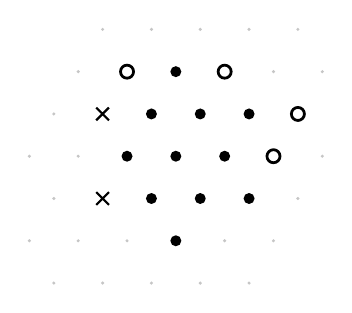
\begin{tikzpicture}[scale=0.62]
\def\pts#1{\foreach \a/\b in {#1} {\fill (\a+0.5*\b, 0.8660254*\b) circle (3.2pt);}}
\def\extra#1{\foreach \a/\b in {#1} {\filldraw[fill=white,line width=1pt] (\a+0.5*\b, 0.8660254*\b) circle (3.8pt);}}
\def\gone#1{\foreach \a/\b in {#1} {\draw[line width=0.8pt] (\a+0.5*\b-0.13, 0.8660254*\b-0.13) -- (\a+0.5*\b+0.13, 0.8660254*\b+0.13) (\a+0.5*\b-0.13, 0.8660254*\b+0.13) -- (\a+0.5*\b+0.13, 0.8660254*\b-0.13);}}
  \foreach \a in {-3,...,3} \foreach \b in {-3,...,3} {
    \pgfmathsetmacro{\x}{\a+0.5*\b}\pgfmathsetmacro{\y}{0.8660254*\b}
    \pgfmathparse{abs(\x)<3.3 && abs(\y)<2.7 ? 1 : 0}
    \ifnum\pgfmathresult=1 \fill[gray!45] (\x,\y) circle (1pt);\fi}
  \pts{0/0,1/0,0/1,-1/1,-1/0,0/-1,1/-1,1/1,-1/2,1/-2,2/-1}
  \gone{-1/-1,-2/1}
  \extra{2/0,0/2,-2/2,2/1}
\end{tikzpicture}
\caption{The set $F$: eleven points of $H$ (black), the two points of $H$ that are left out (crosses), and
four further lattice points (hollow).}
\label{fig:F}
\end{figure}

\subsection{Nine points suffice}
\begin{lemma}\label{lem:nine}
Every set $X$ of fifteen points in the plane with at most seven distances is the vertex set of a regular
$15$-gon or contains nine points with at most six distances.
\end{lemma}

\begin{proof}
Suppose $X$ is not a regular $15$-gon. By Lemma~\ref{lem:hull}, $m\le13$. If the diameter graph restricted
to $X_D$ is not a single cycle, Lemma~\ref{lem:diam}(3) gives an independent set $I$ with
$|I|\ge\lceil m/2\rceil$, and $A=I\cup(X\setminus X_D)$ has $15-\lfloor m/2\rfloor\ge9$ points and at most six
distances. If it is a single cycle and $m\le11$, every other point of the cycle gives
$|A|=15-\frac{m+1}2\ge9$. If it is a single cycle and $m=13$, then $X_D$ is a regular $13$-gon by
Lemma~\ref{lem:C13}, and any nine of its vertices have six distances.
\end{proof}

The regular $15$-gon does need to be excluded: one checks that no nine of its vertices avoid one of its
seven distances.

\subsection{The nine-point sets}
By Proposition~\ref{prop:A} (whose induction covers $n=9$), every nine-point set with at most six distances has
one of the $635$ patterns of $L_9$. They are solved as in Section~\ref{sec:realisations}, with the $56$
principal minors of $G^0$.

\begin{proposition}[computer-assisted]\label{prop:nine}
Of the $635$ patterns of $L_9$, $633$ have finitely many solutions, which give $811$ planar point sets. The
other two have a curve of solutions; they are parametrised by $s\in\R$ (up to finitely many values), with
squared lengths
\[
  1,\ \tfrac{s^2+6s+21}{s^2+3},\ \tfrac{s^2+6s+9}{s^2+3},\ \tfrac{12}{s^2+3},\ \tfrac{s^2+12s+39}{s^2+3}
  \qquad\text{and}\qquad
  1,\ \tfrac{(s-1)^2}4,\ \tfrac{(s+1)^2}4,\ \tfrac{s^2+3}4,\ \tfrac{3s^2+1}4,\ s^2,
\]
and these parametrisations cover every solution.
\end{proposition}

For the two flexible patterns, a lexicographic Gröbner basis of the saturated equations consists of linear
equations and one conic; the parametrisations above are those of the conics, through a rational point,
and they are checked against the basis. Both families consist of genuine point sets for all but finitely many
real $s$.

\subsection{Extending nine points}
\begin{proposition}[computer-assisted]\label{prop:extend15}
Every set of fifteen points with at most seven distances that contains one of the nine-point sets of
Proposition~\ref{prop:nine} has squared distances proportional to $1,3,4,7,9,12,13$.
\end{proposition}

For a nine-point set $K$ with $|\Delta(K)|$ distances the budget is $b=7-|\Delta(K)|\in\{1,2,3\}$, and the
candidate points are found as in Section~\ref{sec:extensions}: a point $y$ added to $K$ is the circumcentre of
three points of $K$, or has squared distances in $\Delta(K)$ to at least $9-2b$ points of $K$. Two cases need more
than Section~\ref{sec:extensions}.

\emph{Collinear triples with budget $3$.} Three nine-point sets have only four distances, and contain three
collinear points. If the points of $K$ at old distances from $y$ include three non-collinear ones, $y$ is
determined as before (all non-collinear triples are used). If they are collinear, they are exactly three
points on a line (no four points of these sets are collinear), so the other six points are at the three new
distances from $y$, each taken exactly twice; then $y$ lies on the perpendicular bisectors of three disjoint
pairs, and two of them that meet determine $y$. When the three bisectors are parallel and distinct there is no
such $y$; when they coincide, $y$ lies on that line and at old distances from the three collinear points, which
gives at most one point for each choice of the three distances.

\emph{The two families.} Write $K(s)$ for the family and work over the field $\Q(s)$. The candidate points of
$K(s)$, constructed as in Section~\ref{sec:extensions} with $s$ as an indeterminate, have coordinates in
$\Q(s)$. None of them has at most $b$ new squared distances to $K(s)$ identically in $s$. A candidate can become
admissible at a particular value $s_0$ only if, among any $b+1$ of its new squared distances, two coincide or
one becomes equal to a squared distance of $K(s_0)$ at $s_0$; this makes $s_0$ a root of an explicit
polynomial. Together with the values of $s$ at which a triple of $K(s)$ becomes collinear, at which a
candidate exists only for special $s$, or at which the coordinates of $K(s)$ degenerate, this gives finitely
many irreducible polynomials with real roots: $209$ for the first family and $135$ for the second.
For each root $s_0$ at which $K(s_0)$ is a genuine point set with the given pattern, $K(s_0)$ is extended exactly
as a rigid set, in the number field $\Q(s_0)$.

\emph{Result.} The fifteen-point sets found in all cases have squared distances proportional to
$1,3,4,7,9,12,13$, and fall into fifteen similarity classes. The computation takes about $16$ minutes on two
cores (program \texttt{fifteen/fifteen.py}).

\begin{proposition}[computer-assisted]\label{prop:palette15}
Up to congruence, there are exactly fifteen sets of fifteen points in the plane all of whose squared distances
lie in $\Pi$: the fourteen sets $E_k$ minus a point, and $F$.
\end{proposition}

The search is that of Proposition~\ref{prop:palette}, now looking for twelve candidate points instead of thirteen.

\begin{proof}[Proof of Theorem~\ref{thm:15}]
Let $X$ be a set of fifteen points with at most seven distances, other than a regular $15$-gon. By
Lemma~\ref{lem:nine} it contains nine points with at most six distances, which by Propositions~\ref{prop:A}
and~\ref{prop:nine} form a set similar to one of the sets of Proposition~\ref{prop:nine}. By
Proposition~\ref{prop:extend15} the squared distances of $X$ are proportional to those of $\Pi$, and by
Proposition~\ref{prop:palette15}, $X$ is similar to $F$ or to $E_k$ minus a point. These sixteen sets are
pairwise non-similar, and $F$ is not similar to a subset of $E_1$ or $E_2$, which by
Theorem~\ref{thm:main} are the only sixteen-point sets with seven distances.
\end{proof}

\begin{remark}
Each of the fifteen sets other than the regular $15$-gon contains a core, so the extension search of
Section~\ref{sec:extensions}, applied to the $282$ cores with five points added instead of six, also finds them;
it finds exactly these fifteen. The regular $15$-gon contains no core.
\end{remark}

\section{A consistency check}\label{sec:check}

The following test uses none of the machinery of Section~\ref{sec:extensions} and could have failed. List the
ten-point subsets of $E_1$ and $E_2$ with at most six distances. Each is a core, so its pattern must be in
$L_{10}$. Moreover, by Theorem~\ref{thm:main}(2) every completion of a core $K$ to sixteen points is a copy of
$E_1$ or $E_2$ placed around $K$, so the number of completions found by the search should be
\[
  \sum_{k=1,2}\frac{\#\{\text{subsets of }E_k\text{ congruent to }K\}\cdot\#\{\text{symmetries of }K\}}
  {\#\{\text{symmetries of }E_k\}}.
\]
The symmetry groups of $E_1$ and $E_2$ have orders $2$ and $6$. The ten-point subsets with at most six
distances fall into $185$ congruence classes with $185$ different patterns, and the predicted numbers of
completions agree with the search of Section~\ref{sec:extensions} pattern by pattern, $826$ in total.

\section{What the proof uses}\label{sec:computation}

\subsection*{Published results}
\begin{enumerate}
\item Theorem~\ref{thm:altman} (Altman; Fishburn), used in Lemma~\ref{lem:hull}.
\item Lemma~\ref{lem:diam}(3), from \cite[Lemmas 3--5 and 9]{W}, used in Proposition~\ref{prop:core}.
\end{enumerate}
Lemma~\ref{lem:diam}(1),(2) and Lemma~\ref{lem:C13} are proved here. No result of \cite{SO} is used; their
Table~9 agrees with our Table~\ref{tab:levels}.

\subsection*{Computations}
\begin{enumerate}
\item Proposition~\ref{prop:lists}: the completeness of the candidate lists (\texttt{generate.py}, about $13$
  minutes on two cores; confirmed by an independent program and, at six points, by a third enumeration)
  and the validity of $527{,}338$ certificates (\texttt{check.py}, about $45$ core-minutes).
\item Proposition~\ref{prop:B}: that the $228$ systems have no solutions besides the $282$ found depends on
  SymPy's Gröbner bases, cross-checked with FLINT; that every solution is realised is checked directly.
  The same applies to Proposition~\ref{prop:nine} (SymPy only).
\item Propositions~\ref{prop:extend} and~\ref{prop:palette} and Corollary~\ref{cor:17}: exhaustive searches
  in exact arithmetic, under a minute together. Propositions~\ref{prop:extend15} and~\ref{prop:palette15}:
  the same kind of search, about $16$ minutes on two cores.
\end{enumerate}
Section~\ref{sec:check} is an independent test of items 2 and 3. The whole classification was also
obtained earlier by a different computation, using certified real-root isolation with msolve in place of
exact number fields; all counts ($228$ patterns, $282$ solutions, $257$ shapes, $185$ extendable patterns,
$826$ completions, two sets) agree.

The notebook \texttt{two-shapes.ipynb} runs Propositions~\ref{prop:B}, \ref{prop:extend}, \ref{prop:palette}
and Corollary~\ref{cor:17} (loading the saved solutions of Proposition~\ref{prop:B} by default and
re-solving a sample; a switch re-solves all $228$ systems in about four minutes), checks the certificates
at four and five points and samples of the others, generates the candidates at five points, carries out
Section~\ref{sec:check}, and checks Section~\ref{sec:fifteen}: the nine-point solutions, the two families, the
extension of a sample of the nine-point sets, Proposition~\ref{prop:palette15}, and the remark at the end of the
section. It was run with Python~3.13 and SymPy~1.14.

\subsection*{Authorship}
Alon Amit posed the problem and directed the research. Claude, an AI model developed by Anthropic, developed
the proofs and the software, carried out the computations and wrote the manuscript. This version replaces an
earlier one (by A.~Amit and GPT-6 Astra), which proved $g(7)=16$ by a related route that relied on the
published enumeration of \cite{SO} and on a computer-assisted proof of the thirteen-cycle lemma; the proof
of Lemma~\ref{lem:hull} is taken from it.

\begin{thebibliography}{99}

\bibitem{A} E. Altman, On a problem of P. Erdős, \emph{Amer. Math. Monthly} \textbf{70} (1963), 148--157.

\bibitem{BY} L.-R. Bao and W.-H. Yu, Constructions of large $m$-distance sets on triangular lattice,
arXiv:2509.00880 (2025).

\bibitem{B} W. T. Budianto, \emph{An observation on 7-distance sets in the Euclidean plane}, master's
thesis, National Central University, Taiwan, 2022.

\bibitem{EF} P. Erdős and P. Fishburn, Maximum planar sets that determine $k$ distances, \emph{Discrete
Math.} \textbf{160} (1996), 115--125.

\bibitem{F} P. Fishburn, Convex polygons with few intervertex distances, \emph{Comput. Geom.} \textbf{5}
(1995), 65--93.

\bibitem{HP} H. Hopf and E. Pannwitz, Aufgabe Nr.~167, \emph{Jahresber. Deutsch. Math.-Verein.}
\textbf{43} (1934), 114.

\bibitem{MP} B. D. McKay and A. Piperno, Practical graph isomorphism, II, \emph{J. Symbolic Comput.}
\textbf{60} (2014), 94--112.

\bibitem{sympy} A. Meurer et al., SymPy: symbolic computing in Python, \emph{PeerJ Comput. Sci.} \textbf{3}
(2017), e103.

\bibitem{SO} F. Szöllősi and P. R. J. Östergård, Constructions of maximum few-distance sets in Euclidean
spaces, \emph{Electron. J. Combin.} \textbf{27}(1) (2020), \#P1.23.

\bibitem{W} X. Wei, A proof of Erdős--Fishburn's conjecture for $g(6)=13$, \emph{Electron. J. Combin.}
\textbf{19}(4) (2012), \#P38.

\end{thebibliography}

\appendix
\section{The certificate checker}\label{app:check}

The following functions from \texttt{certificates/check.py} verify one certificate. A polynomial is a
dictionary mapping exponent tuples to integer coefficients; a pattern is the list of colours of the pairs
$(0,1),(0,2),\dots,(n-2,n-1)$. The rest of the file reads certificates, one JSON object per line, and runs
\texttt{check} on each.

\lstinputlisting[firstline=24,lastline=101]{../certificates/check.py}

\end{document}
